\documentclass[display,bioinf]{pptex}

\setfootline{Ulrich Bodenhofer}

\begin{document}
\begin{slide}
\titleslide[Ulrich Bodenhofer\\
ulrich.bodenhofer@scch.at \\
+43 7236 3343 832 \\
www.scch.at]{PP\TeX}{A Short Demo}
\end{slide}

\begin{slide}
\simpletextslide{Standard Itemization}{%
\begin{itemize}
\item Mama got a sqeezebox\dots
\item daddy
\item never sleeps
\item at night
\end{itemize}}
\end{slide}

\begin{slide}
\stepwise{\simpletextslide{Standard Itemization (animated)}{%
\step{\begin{itemize}
\item Mama got a sqeezebox\dots
\step{\item daddy}
\step{\item never sleeps}
\step{\item at night}
\end{itemize}}}}
\end{slide}

\begin{slide}
\simpleslide{Left \&\ Right:\newline Central Dogma of Molecular Biology}{%
\defaulttextboxleft{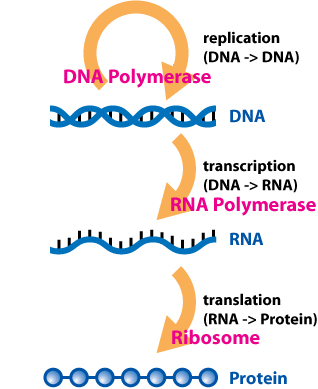
\includegraphics[width=0.8\textwidth]{Central_Dogma}}
\defaulttextboxright{%
DNA makes RNA makes proteins:
\begin{itemize}
\item DNA is {\em transcribed} into RNA in the nucleus
\item RNA is {\em translated} into an amino acid sequence in a ribosome
\end{itemize}}}
\end{slide}

\begin{slide}
\stepwise{\simpleslide{Left \&\ Right:\newline Central Dogma of Molecular Biology}{%
\defaulttextboxleft{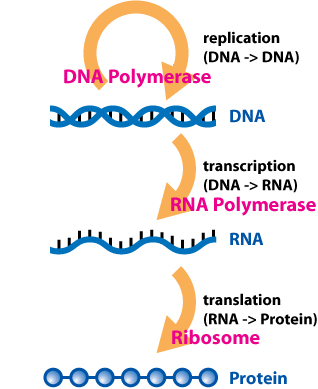
\includegraphics[width=0.8\textwidth]{Central_Dogma}}
\step{\defaulttextboxright{%
DNA makes RNA makes proteins:
\begin{itemize}
\item DNA is {\em transcribed} into RNA in the nucleus
\item RNA is {\em translated} into an amino acid sequence in a ribosome
\end{itemize}}}}}
\end{slide}

\begin{slide}
\stepwise{\simpleslide{Left \&\ Right:\newline Central Dogma of Molecular Biology}{%
\step{\defaulttextboxright{%
DNA makes RNA makes proteins:
\begin{itemize}
\item DNA is {\em transcribed} into RNA in the nucleus
\item RNA is {\em translated} into an amino acid sequence in a ribosome
\end{itemize}}}
\step{\defaulttextboxleft{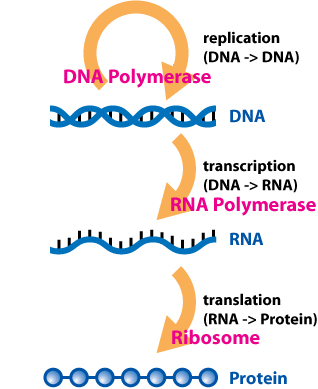
\includegraphics[width=0.8\textwidth]{Central_Dogma}}}}}
\end{slide}


\end{document}
